% compress:  compresses the navigation bar                                      
% trans | handout:  restrict overlays
%\documentclass[dvips,xcolor=cmyk]{beamer}
\documentclass[xcolor=cmyk]{beamer}
%\documentclass[pdftex,compress,xcolor=cmyk,trans]{beamer}

% % force compression of graphic objects?  I need to research this more, JJS
% 4/24/12
% \pdfminorversion=5
% \pdfcompresslevel=9
% \pdfobjcompresslevel=2

%% Packages
\usepackage{amsmath,amssymb}
\usepackage{enumerate}
%\usepackage{graphics}
\usepackage{array}
\usepackage{psfrag}
%\usepackage{subfigure}
\usepackage{graphicx}
\usepackage{subfig}
%\usepackage{movie15} % separate package with good integration with Beamer
\usepackage{sidecap}
\usepackage{caption}

%\usepackage[driverfallback=dvipdfm]{hyperref}

%\usepackage{easymovie}             
\usepackage[normalem]{ulem}

\usepackage{natbib,natbibspacing}
%\newcommand{\newblock}{}

%\usepackage{enumitem}

\usepackage{pstricks}
%\usepackage{tikz}
%\usetikzlibrary{positioning}
%\usetikzlibrary{calc}
\usepackage{nameref}
\usepackage{url}

\usepackage[T1]{fontenc}
\usepackage{arev}
\usepackage{type1cm}  

\usepackage{setspace}  

\captionsetup{font=scriptsize,labelfont=scriptsize}
%\setlength{\parindent}{0.3in}
%\setlength{\parskip}{0.1in}

% commands not needed for math

%% Set formatting to conform to NREL standards
% NREL "signature" colors
\definecolor{nrelblue}{cmyk}{1,0.44,0,0}
\definecolor{nrelyellow}{cmyk}{0,0.42,1,0.01}
\definecolor{nrelgreen}{cmyk}{0.56,0,1,0.27}
\definecolor{nrelred}{cmyk}{0,0.74,1,0.47}
\definecolor{nrelgray}{cmyk}{0.11,0.01,0,0.64}
% NREL "secondary" colors -- double check these !! JJS 4/21/12
\definecolor{nrellightblue}{cmyk}{0.9,0.11,0,0}
\definecolor{nrellightyellow}{cmyk}{0,0.24,94,0}
\definecolor{nrellightgreen}{cmyk}{0.50,0,1,0}
\definecolor{nrellightred}{cmyk}{0,0.79,1,0.11}
\definecolor{nrellightgray}{cmyk}{0.02,0,0,0.18}

\input basic.ltx
\def\directory{EPSF/}

% custom defined colors
\definecolor{foottextcolor}{named}{white}

% set beamer theme(s)
\usecolortheme[named=nrelblue]{structure}
% \usefonttheme[onlymath]{serif}  % use sans serif for text, but serif for
% math

\newlength{\lrmargin} % left and right margin width
\setlength{\lrmargin}{1em}
\setbeamersize{text margin left=\lrmargin}
\setbeamersize{text margin right=\lrmargin}

\setbeamertemplate{navigation symbols}{}  % gets rid of navigation symbols

% change the default footnote font size
\usepackage{etoolbox}
\makeatletter
\patchcmd{\@makefntext}{\insertfootnotetext{#1}}{\insertfootnotetext{\tiny#1}}{}{}
\makeatother

% define frame-title template
\setbeamertemplate{frametitle}
{
  \textbf{\Large \insertframetitle}
  \par
  \vspace{-0.5ex}
  \mbox{\hspace{-\lrmargin}\rule{\paperwidth}{0.2ex}}
}
\setbeamertemplate{footline}
{
  \colorbox{nrelblue}{\parbox{0.99\paperwidth}{
      \color{foottextcolor} \Tiny
      \hspace{\stretch{0.05}} NATIONAL RENEWABLE ENERGY LABORATORY \hfill
\textbf{\insertframenumber}\hspace{\stretch{0.1}} }}
}

% specify subitem to be a circle
\setbeamertemplate{itemize subitem}[circle]

%% define a ``listheader'' format
\newcommand{\listhead}[1]{{\color{nrelblue}\textbf{#1}}}
%\newcommand{\listhead}[1]{\textbf{#1}}

%% define a custom itemize environment with adjusted spacing
\newenvironment{myitemize}[1][]{\begin{itemize}[#1]\addtolength{\itemsep}{1ex}}{\end{itemize}}

\newcommand{\uvec}[1]{\bar{#1}}
\newcommand{\tens}[1]{\underline{\underline{#1}}}
\renewcommand{\vec}[1]{\underline{#1}}
\renewcommand{\skew}[1]{\widetilde{#1}}


\begin{document}

%
{\setbeamercolor{normal text}{fg=white,bg=nrelblue}
  \usebeamercolor[fg]{normal text}
\begin{frame}[plain]{test}

\rput[tl](-0.2,2.2){
\includegraphics[width=0.2\textwidth,clip]{nrel_logo_white.eps}}

\rput[tl](3.4,2.1){\parbox{\textwidth}{
\textbf{Partitioned Nonlinear Structural Analysis  \\
 of Wind Turbines using BeamDyn } } }

\rput[tl](-0.5,1.0){
\includegraphics[width=1.1\textwidth,clip]{nrel_photo_bar.eps}
}

\rput[tl](2.0,-0.5){\parbox{\textwidth}{  \normalsize
Qi Wang,  Michael A. Sprague\\
 Jason Jonkman, Bonnie Jonkman
}}

\rput[tl](2.0,-1.2){\parbox{0.8\textwidth}{\footnotesize
National Renewable Energy Laboratory\\
}}

\rput[tl](2.0,-1.8){\parbox{\textwidth}
{AIAA SciTech 2016\\San Diego, CA\\
4--8 January 2016}}

\rput[tl](0.0,-3.2){\parbox{\textwidth}{
{
\begin{spacing}{0.6}
\tiny NREL is a national laboratory of the U.S.\ Department of Energy,
Office of
Energy Efficiency and Renewable Energy, 
operated by the Alliance for Sustainable Energy, LLC.
\end{spacing}
}}} 

\psline[linewidth=1pt,linecolor=white](-1,-4.9)(8,20)

\psline[linewidth=1pt,linecolor=white](-1,-2.0)(11,20) 
   

 \end{frame}
}

%------------------------------------------------------------------------------
\begin{frame}{Motivation}
  \begin{itemize}
    \item
    Beam model currently used in FAST
    \begin{itemize}
      \item
      Euler-Bernoulli beam model with shortening effect
      \item
      Two degree-of-freedoms
      \item
      Assumed-mode method
    \end{itemize}
    \item
    Beam models used in other wind turbine tools
    \begin{itemize}
        \item
        Multibody-formulation
        \item
        Linear beam models
        \item
        Constraints introduced between linear beams to describe large deflections and rotations
        \item
        Finite element method
    \end{itemize}
    \item
    Partitioned Analysis
    \begin{itemize}
        \item FAST modularization framework
        \item Tight coupling
        \item Loose coupling
    \end{itemize}
  \end{itemize}
\end{frame}
%------------------------------------------------------------------------------

%------------------------------------------------------------------------------
\begin{frame}{Objective}
    \normalsize
    \begin{itemize}
    \item
    Objective: create efficient high-fidelity beam models for wind turbine blade analysis that 
      \begin{itemize}
          \item
          Based on Geometrically Exact Beam Theory (GEBT) 
          \item
          Advanced numerical technique for implementation
          \item
          Achieve the speed of computational design without significant loss of accuracy comparing to the ultimate accuracy obtained by 3D nonlinear FEA
          \item
          Compatible with the FAST modularization framework
          \item
          Verification and Validation
      \end{itemize}
    \end{itemize}
    \includegraphics[width=0.4\textwidth,clip=true]{figs/static_test.eps}
\hspace{0.05in}
\includegraphics[width=0.18\textwidth,clip=true]{figs/dyn_test.eps}

\rput[tl](7.6,2.5){\parbox{0.35\textwidth}{\small NWTC static and dynamic
blade tests showing typical large, elastic deflections.}}
\end{frame}
%------------------------------------------------------------------------------

%------------------------------------------------------------------------------
\begin{frame}{Approach}
  \begin{itemize}
    \item
    Implementation
    \begin{itemize}
      \item
      Geometrically Exact Beam Theory (GEBT) 
      \begin{itemize}
        \item
        \pause
        First proposed in 1973 \citep{Ressiner1973}
        \item
        \pause
        Extended to composite beams \citep{HodgesBeamBook}
        \item
        \pause
        Displacement-based implementation \citep{Bottasso:1998,Dymore:2013}
        \item
        \pause
        Mixed implementation \citep{YuGEBT,Wang:GEBT2013}
      \end{itemize}
      \item
      Legendre Spectral Finite Element (LSFE) \citep{Patera:1984}
      \begin{itemize}
          \item
          \pause
          A $p$-version high-order finite element 
          \item
          \pause
          Successfully applied to simulation of fluid dynamics, geophysics, elastodynamics
          \item
          \pause
          Limited usage in structural dynamics
      \end{itemize}
      \item
      FAST Modularization Framework \citep{Jonkman:2013}
      \begin{itemize}
          \item Loose coupling
          \item Predictor-correction          
      \end{itemize}
    \end{itemize}
    \item
    BeamDyn, an alternative of ElastoDyn in FAST
  \end{itemize}
\end{frame}
%------------------------------------------------------------------------------

%------------------------------------------------------------------------------
\begin{frame}{GEBT}
\begin{itemize}
    \item Governing Equation
      \begin{align*} 
      \dot{\underline{h}} - \underline{F}^\prime &= \underline{f} \\
      \dot{\underline{g}} + \dot{\widetilde{u}} \underline{h} -
      \underline{M}^\prime - (\widetilde{x}_0^\prime + \widetilde{u}^\prime) \underline{F}
      &= \underline{m} 
      \end{align*}
    
    \item Constitutive Equation
    \begin{columns}[c]
      \column{2.0 in}
      
      \begin{align*}
      \begin{Bmatrix} \underline{h} \\ \underline{g} \end{Bmatrix} &=
      \underline{\underline{\mathcal{M}}} \begin{Bmatrix} \dot{\underline{u}} \\
      \underline{\omega} \end{Bmatrix} \\
      \begin{Bmatrix} \underline{F} \\ \underline{M} \end{Bmatrix} &=
      \underline{\underline{\mathcal{C}}} \begin{Bmatrix} \underline{\epsilon} \\
      \underline{\kappa} \end{Bmatrix} 
      \end{align*}
      \column{2.0 in}
      \begin{itemize}
        \scriptsize
        \pause
        \item
        $\tens{\mathcal{M}}$ and $\tens{\mathcal{C}}$ are $6 \times 6$ sectional mass and stiffness matrices, respcetively \pause
        \item
        Elastic couplings are captured \pause
        \item
        Timoshenko-like beam model
      \end{itemize}
      
      \end{columns}

    \item Strain Measures
    
    \begin{columns}[c]
    \column{2.0 in}
      \begin{equation*}
      \label{1DStrain}
      \begin{Bmatrix}
          \vec{\epsilon} \\
          \vec{\kappa}
      \end{Bmatrix}
      =
      \begin{Bmatrix}
          \vec{x}^\prime_0 + \vec{u}^\prime - (\tens{R} ~\tens{R}_0) \bar{\imath}_1 \\
          \vec{k} 
      \end{Bmatrix}
      \end{equation*}   
      
      \column{2.0 in}
        \begin{itemize}
        \scriptsize
          \pause
          \item
          Geometrically exact: deformed beam geometry is represented exactly
          \pause
          \item 
          Small strains
        \end{itemize}
      \end{columns}
    \end{itemize}

\end{frame}
%------------------------------------------------------------------------------

%------------------------------------------------------------------------------
\begin{frame}{Legendre Spectral Finite Elements}
\normalsize

\begin{itemize}
\item
LSFE methods combine the geometric flexibility of
the FE method with the accuracy of global spectral methods.
%
\begin{itemize}
%
   \item Solution improved through increased basis polynomial order
($p$-refinement)
%
    \item LSFEs employ Lagrangian interpolant shape functions with nodes at
Gauss-Lobatto-Legendre (GLL) points 
%    \item Early SFEs employed Chebyshev-based shape functions; largely
%abandoned in favor of more straight-forward and efficient Legendre-based
%elements
%
  \item \textit{Exponential} convergence rates for sufficiently
smooth solutions

\end{itemize}
%
%  \item SFEs should not be confused with what are known as \textit{spectral
%elements}, or \textit{modal spectral elements},
%in the structural analysis community (\eg, Doyle 1997)

\item Numerical Integration
    \begin{itemize}
        \item Gauss Integration
        \item Trapezoidal-Rule Integration
    \end{itemize}

\end{itemize}

\begin{figure}[h!tp]
   \psfrag{note}[][]{$p$ refine}
   \psfrag{p1}[][]{$N=1$}
   \psfrag{p2}[][]{$N=4$}
   \includegraphics[width=0.5\textwidth,clip]{figs/refine.eps}
\end{figure}


\end{frame}

%------------------------------------------------------------------------------

%------------------------------------------------------------------------------
\begin{frame}{Partitioned Analysis}
   \begin{itemize}
       \item
       System Decomposition
       \item
       Coupled System
       \item
       Loose coupling
       \item
       Module Coupling Algorithm \pause
       \begin{enumerate}

\item Using linear or quadratic extrapolation of known inputs, approximate the inputs at $t+\Delta t$.  \pause

\item Update the states of all modules to $t + \Delta t$.  \pause

\item Solve the global system of input-output equations at $t + \Delta t$.  Depending on the relationship between modules and the module output equations, this system solve can range from a simple transfer of information to a full nonlinear-system solve. \pause

\item Either accept the states, inputs, and outputs, or apply a correction by repeating step (2) with the inputs calculated in Step (3), and then repeating Step (3).

\end{enumerate}

       
   \end{itemize}
\end{frame}
%------------------------------------------------------------------------------

%------------------------------------------------------------------------------
\begin{frame}{Example 1: Partitioned Analysis}

   \begin{itemize}
    \item 
    Beam-Spring-Damper-Mass System
    \begin{center}
    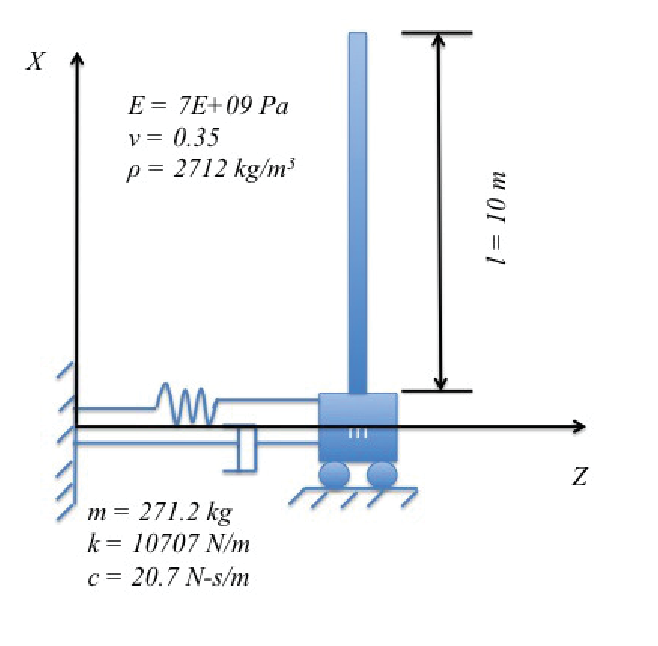
\includegraphics[width=2.0in]{EPSF/CoupledSystem.eps}
    \end{center}
    \begin{itemize}
        \item
        Time integrator for SDM: Adams-Bashforth-Moulton (ABM4)
        \item
        Time integrator for beam: Generalized-$\alpha$
        \item
        Benchmark: ANSYS 60 BEAM188 elements; $10^{-5}$s time increment
    \end{itemize}
    \end{itemize}
    

\end{frame}
%------------------------------------------------------------------------------

%------------------------------------------------------------------------------
\begin{frame}{Example 1: Partitioned Analysis}
\begin{itemize}
    \begin{columns}[c]
        \column{2.3in}
        \item $Root~Displacement$\\
        \linebreak[4]\\
          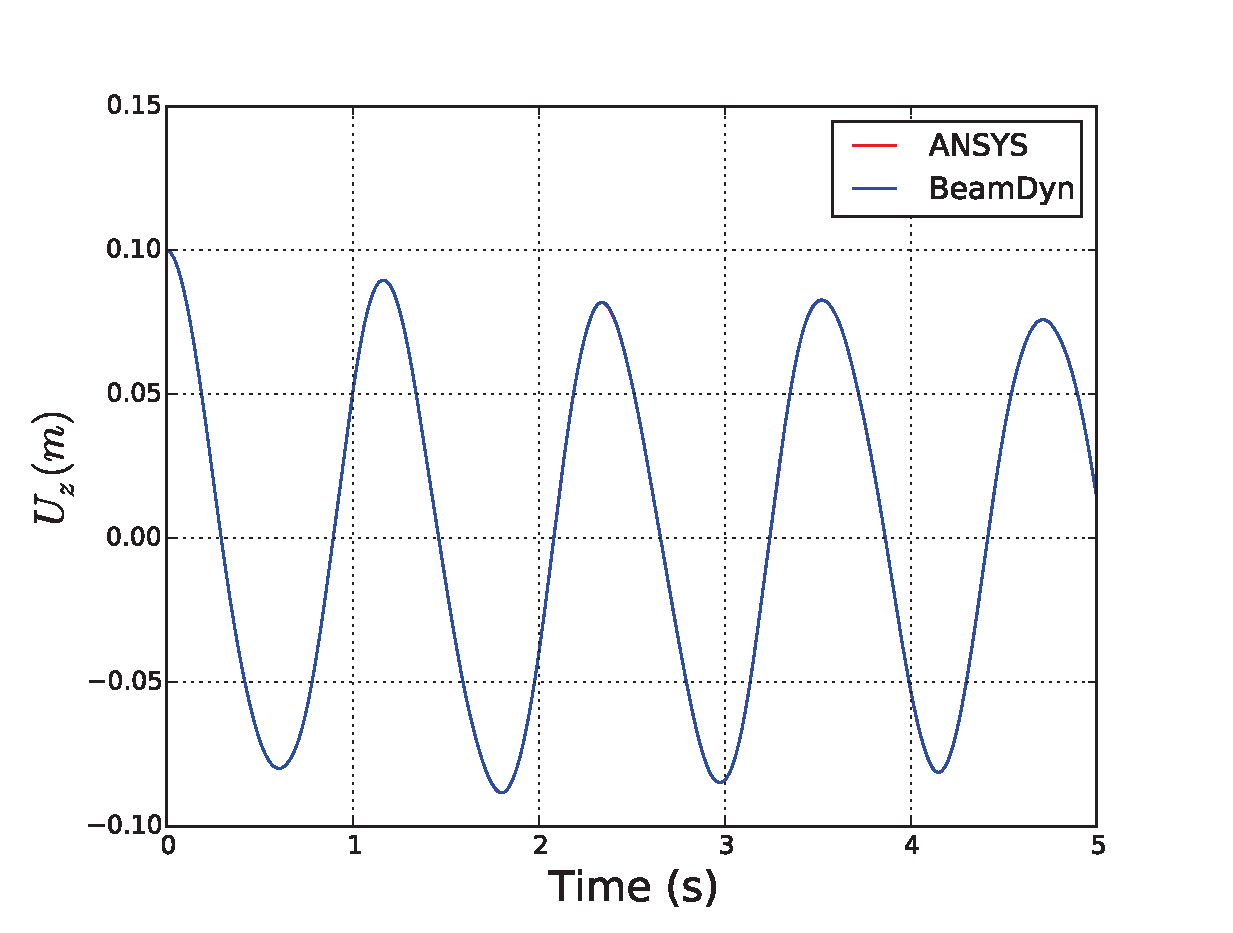
\includegraphics[width=1.7in]{EPSF/Disp_Root.eps}\\
          \item $Root~Velocity$\\
          \linebreak[4]
           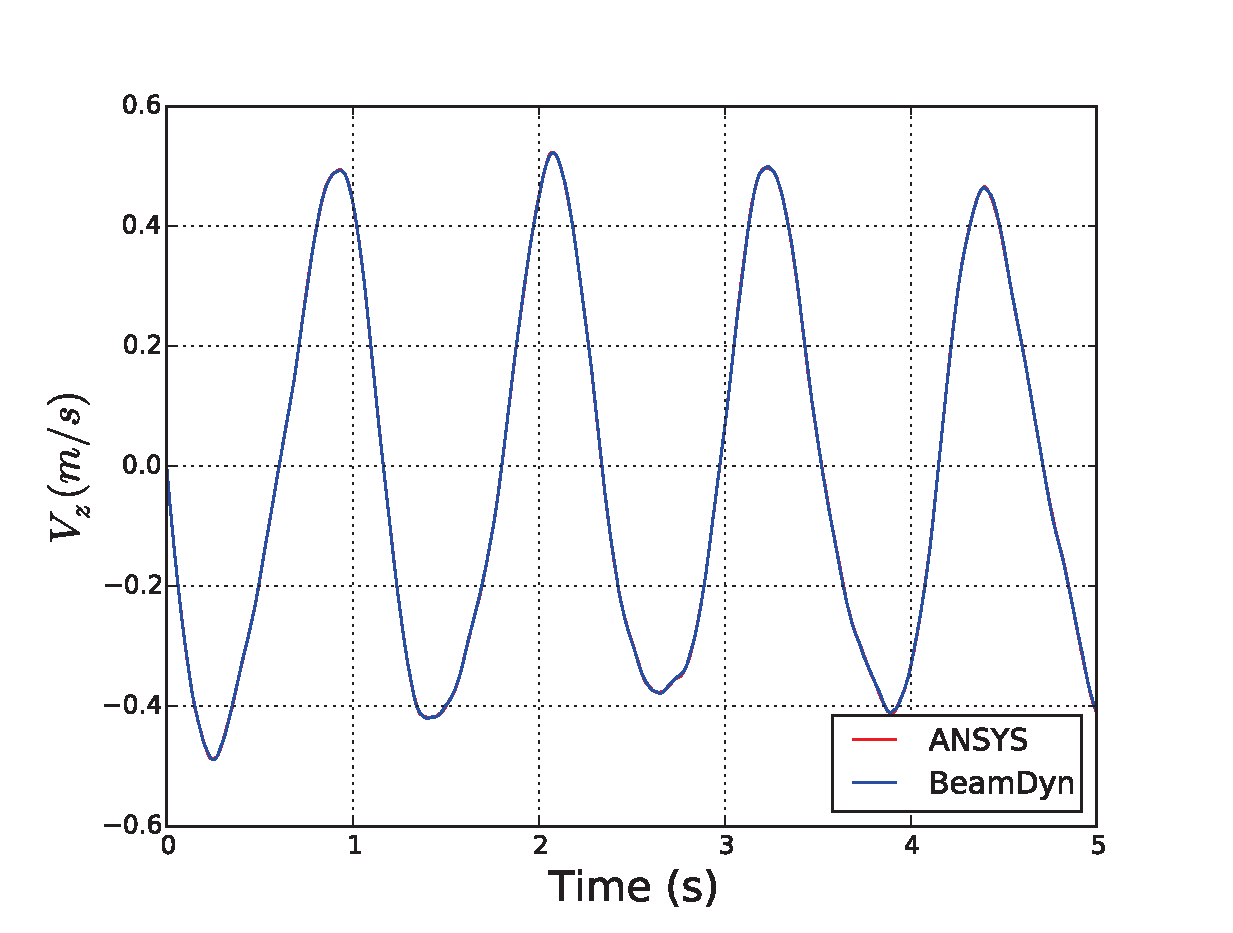
\includegraphics[width=1.7in]{EPSF/Vel_Root.eps}
         \column{2.3in} 
         \item $Tip~Displacement$\\
        \linebreak[4]
           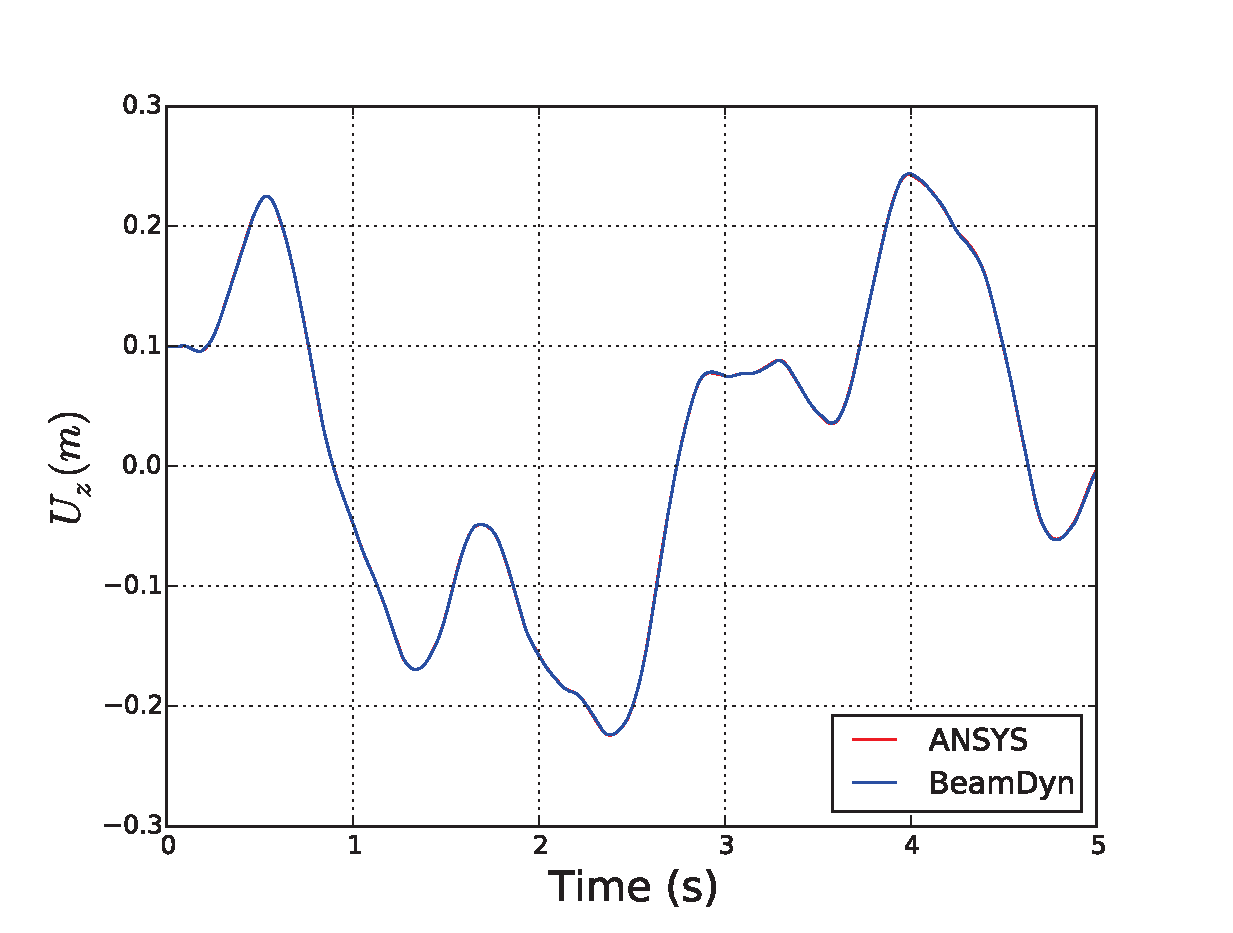
\includegraphics[width=1.7in]{EPSF/Disp_Tip.eps}\\
          \item $Root~Acceleration$\\
          \linebreak[4]
           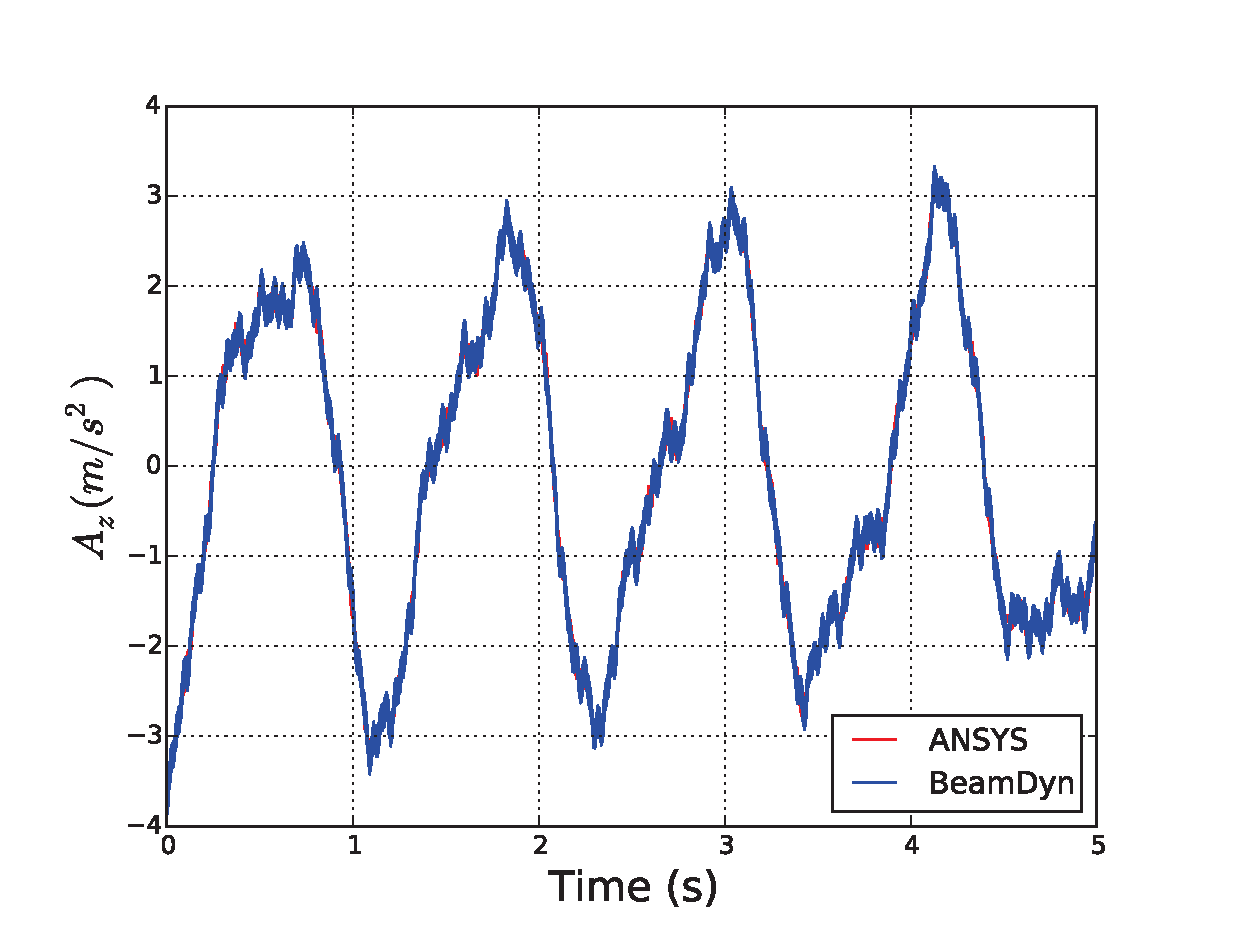
\includegraphics[width=1.7in]{EPSF/Acc_Root.eps} 
    \end{columns}
    
\end{itemize}
\end{frame}
%------------------------------------------------------------------------------



%------------------------------------------------------------------------------
\begin{frame}{Example 1: Partitioned Analysis}
    \begin{itemize}
        \begin{columns}[c]
            \column{2.3in}
            \item Stability \\
            \linebreak[4]\\
            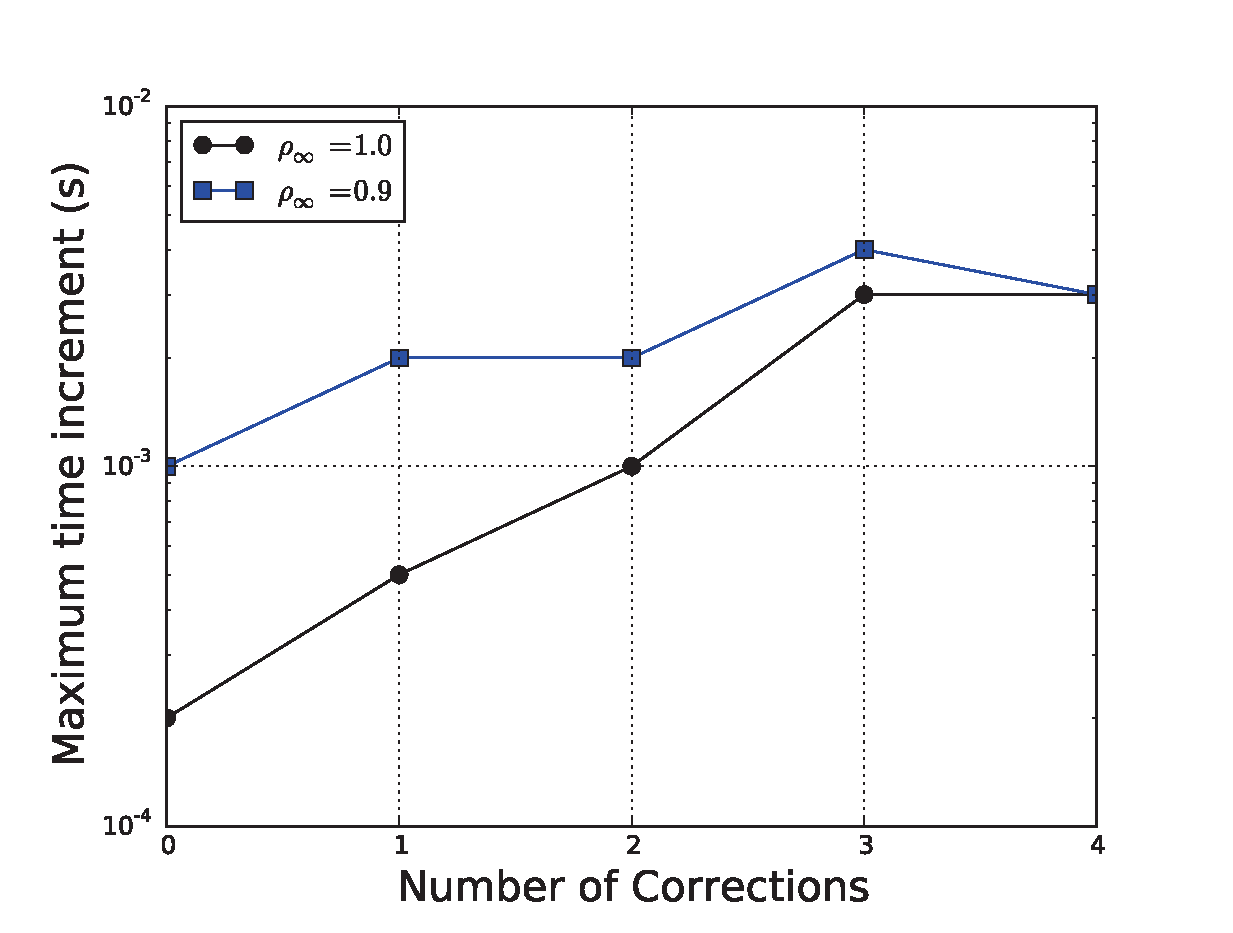
\includegraphics[width=2.0in]{EPSF/dt_pc.eps}
            \column{2.3in}
            \item Accuracy \\
            \linebreak[4]\\
            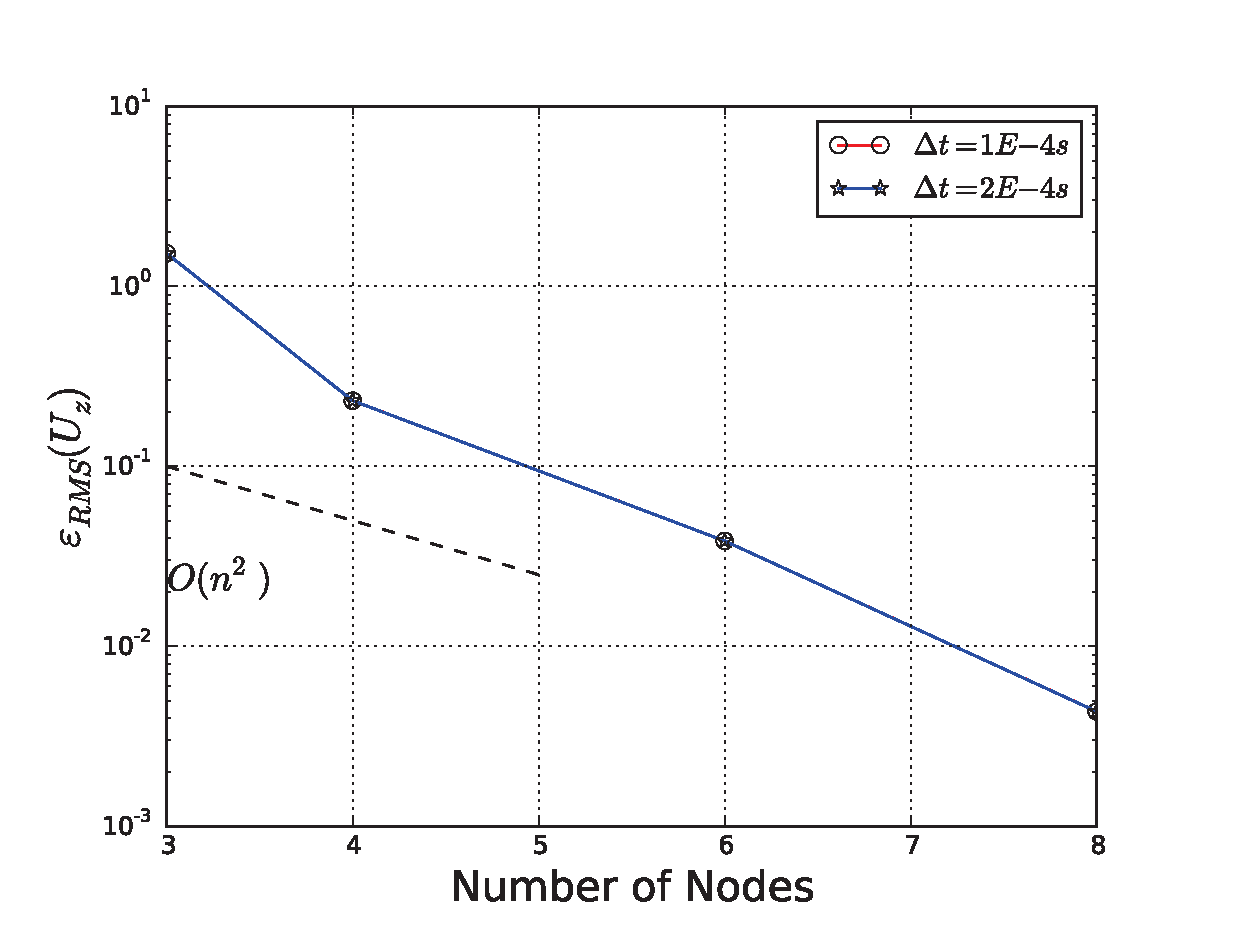
\includegraphics[width=2.0in]{EPSF/RMS_dt_node.eps}
        \end{columns}
        \item
        Corrections and numerical damping help maximum allowable time step size
        \item
        RMS Error
        \begin{equation*}
\varepsilon_{RMS}=\sqrt{\frac{\sum_{k=0}^{n_{max}}[U_z^k-U_b(t^k)]^2}{\sum_{k=0}^{n_{max}}[U_b(t^k)]^2}}
\label{RMSdefi}
\end{equation*} 
        
    \end{itemize}
\end{frame}
%------------------------------------------------------------------------------

%------------------------------------------------------------------------------
\begin{frame}{Example 2: NREL 5-MW Wind Turbine}
     \begin{itemize}
         \item NREL 5-MW Wind Turbine
             \begin{itemize}
                 \item 61.5m long with initial twist
                 \item 49 cross-sectinoal stations
             \end{itemize}
        \begin{columns}[c]
            \column{2.5in}
            \item Tip Displacement
            
             \linebreak[4]\\
            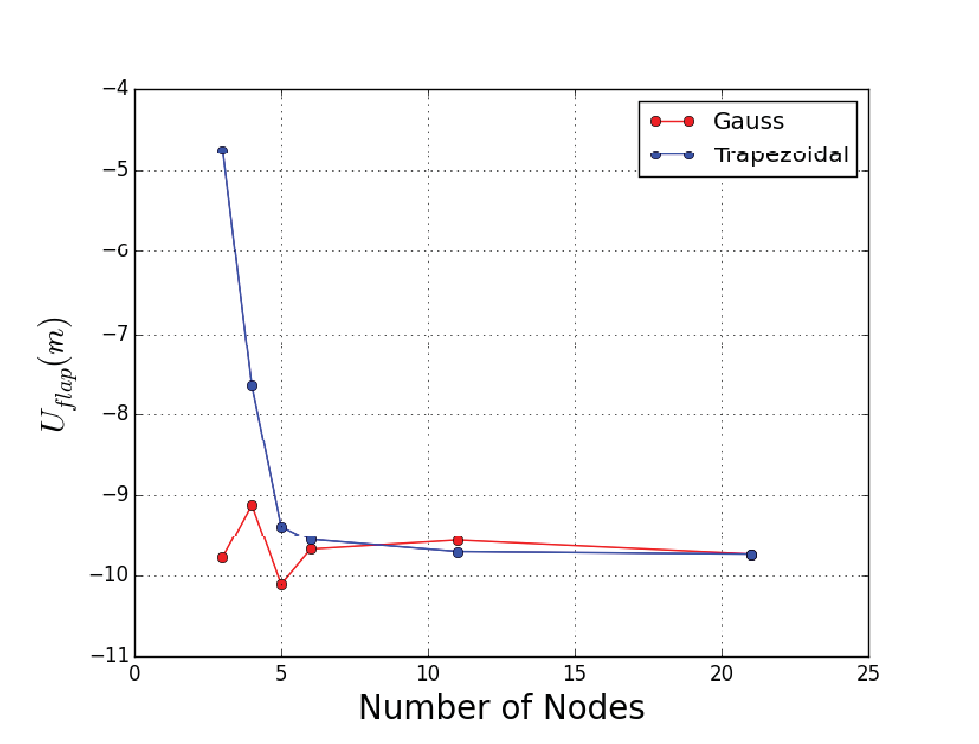
\includegraphics[width=2.5in]{EPSF/5MW_Static_Tip.eps}
            
            \column{2.5in}    
             \item Blade Mass
             \linebreak[4]\\
            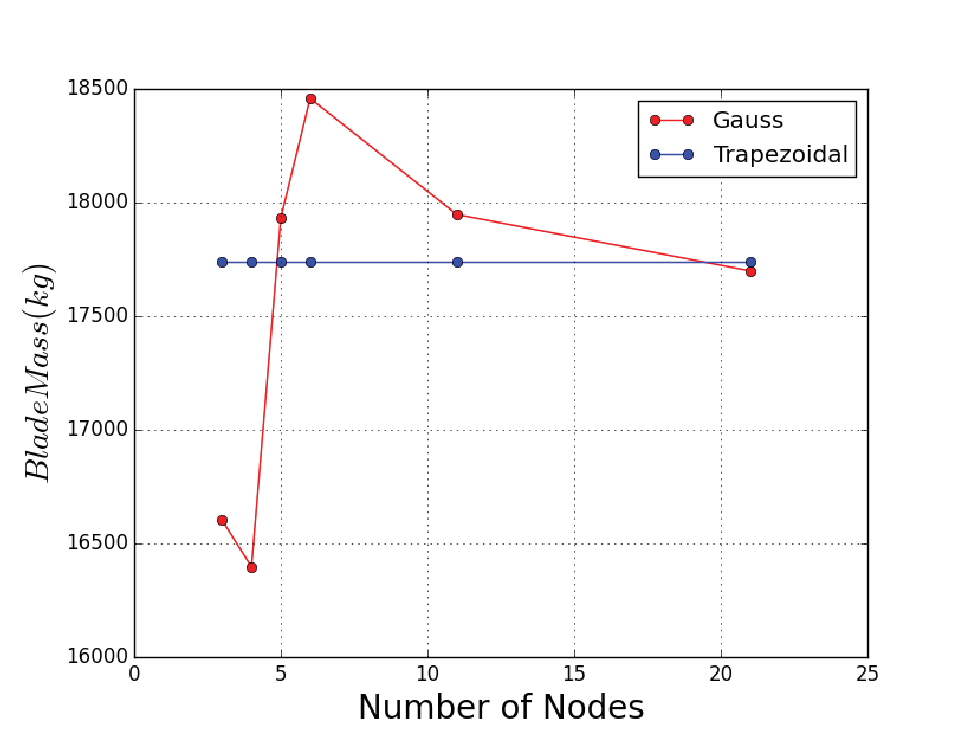
\includegraphics[width=2.5in]{EPSF/5MW_Mass_Scaled.eps}
        \end{columns}
    \end{itemize}  
\end{frame}
%------------------------------------------------------------------------------


%------------------------------------------------------------------------------
\begin{frame}{Example 2: NREL 5-MW Wind Turbine}
    \begin{itemize}
        \item
        Time Discretization
%         \linebreak[4]\\
         \begin{center}
         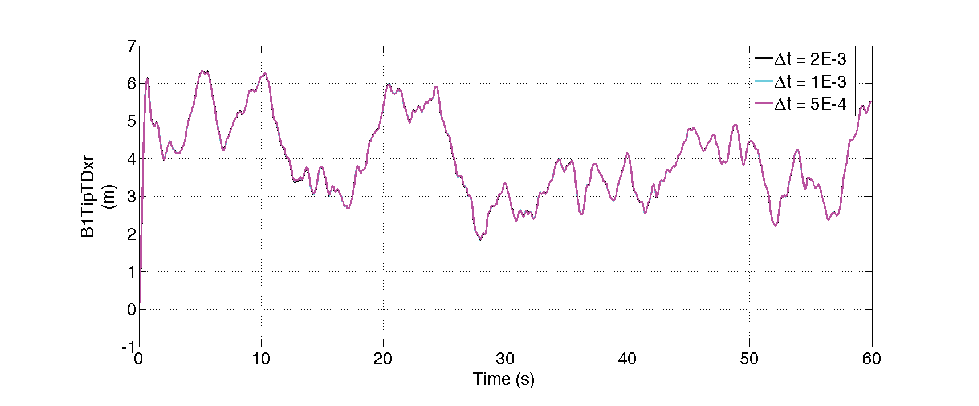
\includegraphics[width=3.3in]{EPSF/5MW_Coupled_dt.eps}
         \end{center}
         \item
         Space Discretization
%         \linebreak[4]\\
         \begin{center}
         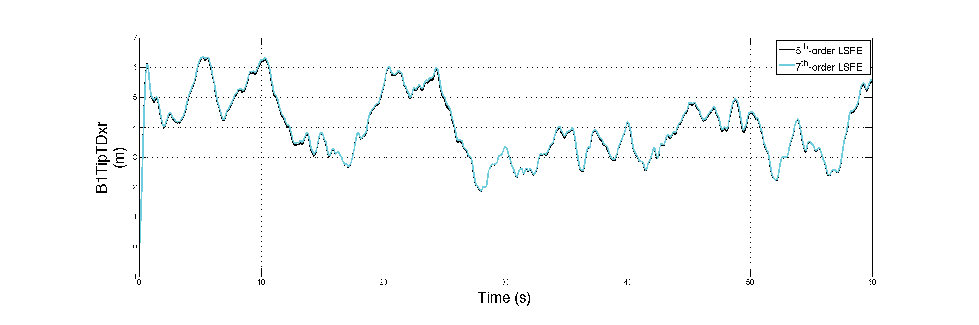
\includegraphics[width=3.5in]{EPSF/5MW_Coupled_Mesh.eps}
         \end{center}
    \end{itemize}
\end{frame}
%------------------------------------------------------------------------------

%------------------------------------------------------------------------------
\begin{frame}{Example 2: NREL 5-MW Wind Turbine}
    \begin{itemize}
        \item
        Aero-Servo-Elastic Coupled Analysis
        \item 
        Mean Wind Speed 12 $m/s^2$ with Turbulence
        \item
        Test Case 26 in FAST Archive
        
         \item Tip Displacement $U_{flap}$
         \begin{center}
         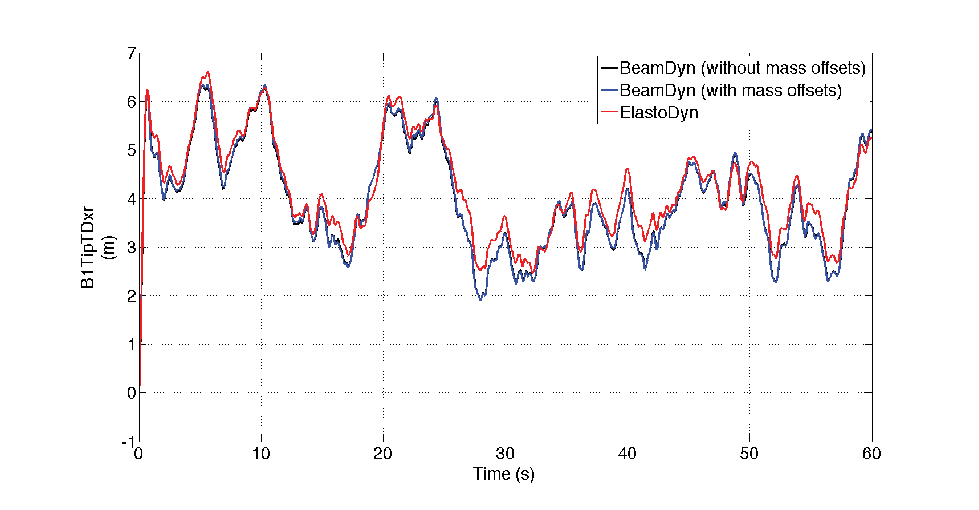
\includegraphics[width=4.5in]{EPSF/B1TipTDxr.eps}
         \end{center}
    \end{itemize}
\end{frame}
%------------------------------------------------------------------------------

%------------------------------------------------------------------------------
\begin{frame}{Example 2: NREL 5-MW Wind Turbine}
    \begin{itemize}
        \item
        Tip Displacement $U_{edge}$
         \begin{center}
         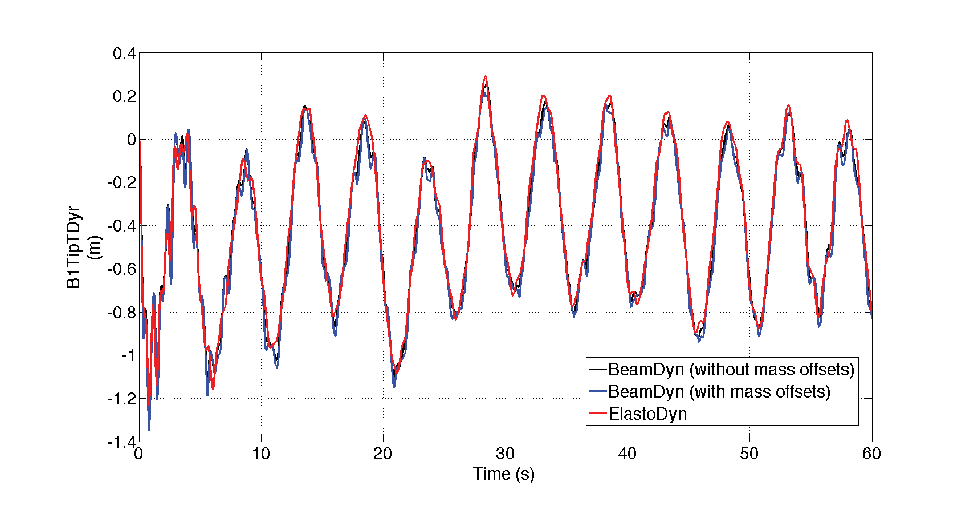
\includegraphics[width=2.7in]{EPSF/B1TipTDyr.eps}
         \end{center}
         \item
         Tip Displacement $U_{axial}$
         \begin{center}
         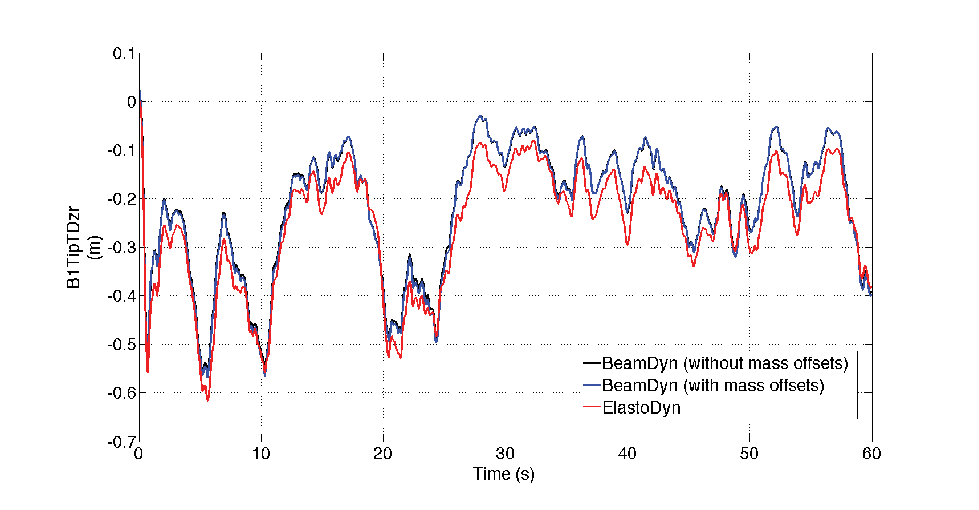
\includegraphics[width=2.7in]{EPSF/B1TipTDzr.eps}
         \end{center}
    \end{itemize}
\end{frame}
%------------------------------------------------------------------------------

%------------------------------------------------------------------------------
\begin{frame}{Example 2: NREL 5-MW Wind Turbine}
    \begin{itemize}
        \item
        Root Reaction Force $F_{flap}$
         \begin{center}
         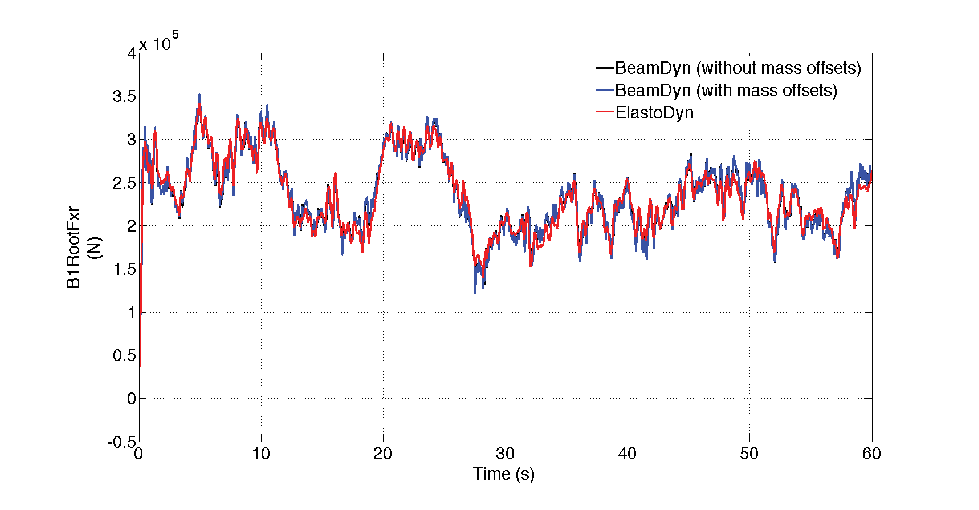
\includegraphics[width=2.7in]{EPSF/B1RootFxr.eps}
         \end{center}
         \item
         Root Reaction Force $F_{edge}$
         \begin{center}
         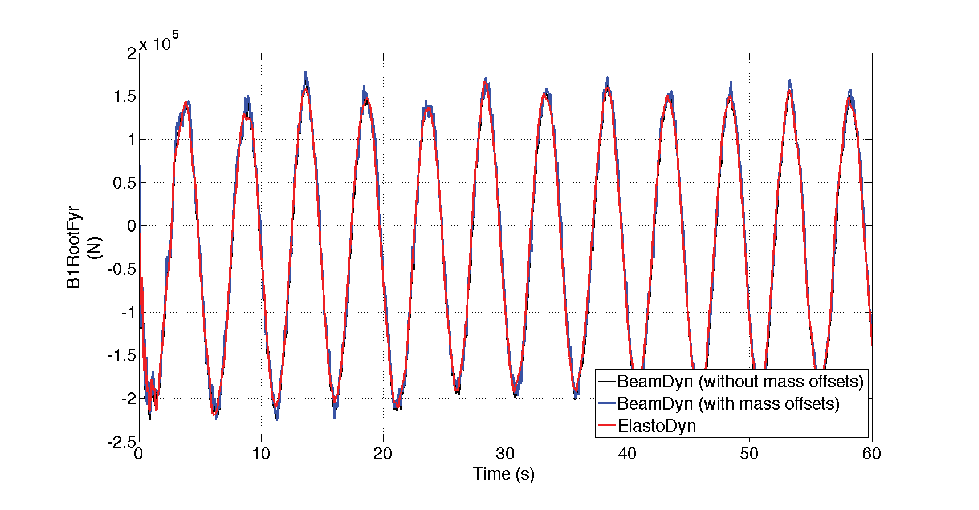
\includegraphics[width=2.7in]{EPSF/B1RootFyr.eps}
         \end{center}
    \end{itemize}
\end{frame}
%------------------------------------------------------------------------------

%------------------------------------------------------------------------------
\begin{frame}{Example 2: NREL 5-MW Wind Turbine}
    \begin{itemize}
        \item
        Root Reaction Force $F_{axial}$
         \begin{center}
         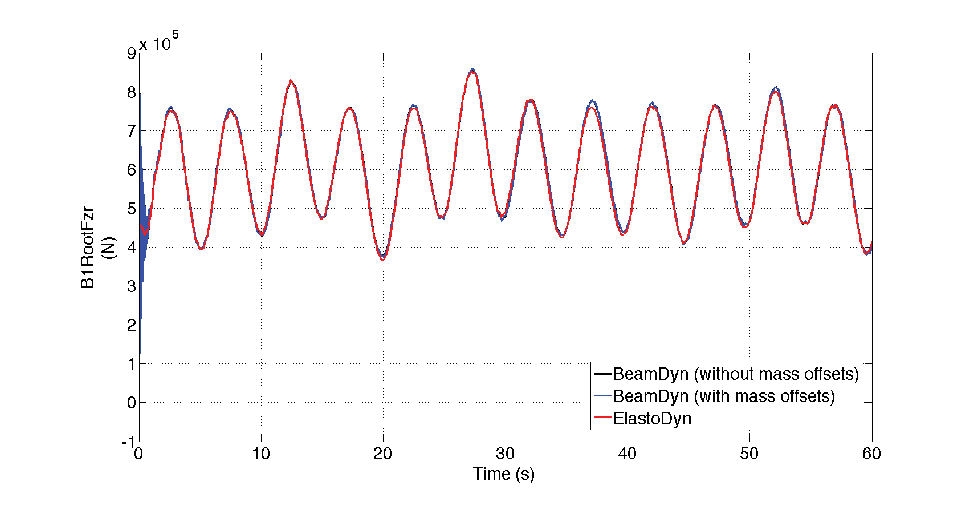
\includegraphics[width=2.7in]{EPSF/B1RootFzr.eps}
         \end{center}
         \item
         Root Reaction Moment $M_{edge}$
         \begin{center}
         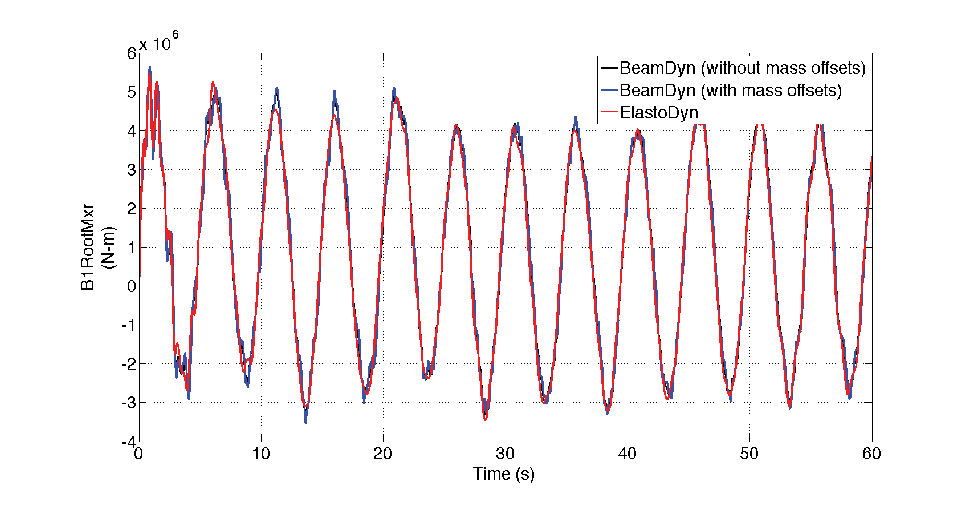
\includegraphics[width=2.7in]{EPSF/B1RootMxr.eps}
         \end{center}
    \end{itemize}
\end{frame}
%------------------------------------------------------------------------------

%------------------------------------------------------------------------------
\begin{frame}{Example 2: NREL 5-MW Wind Turbine}
    \begin{itemize}
        \item
        Root Reaction Moment $M_{falp}$
         \begin{center}
         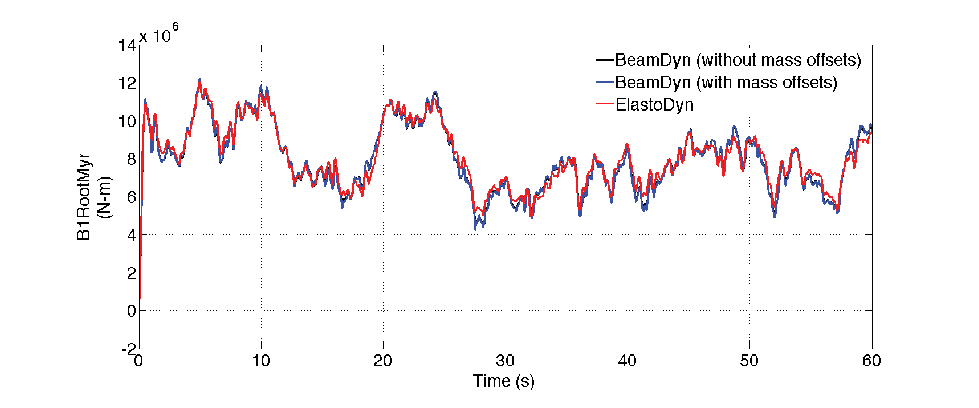
\includegraphics[width=2.8in]{EPSF/B1RootMyr.eps}
         \end{center}
         \item
         Root Reaction Torque $M_{pitch}$
         \begin{center}
         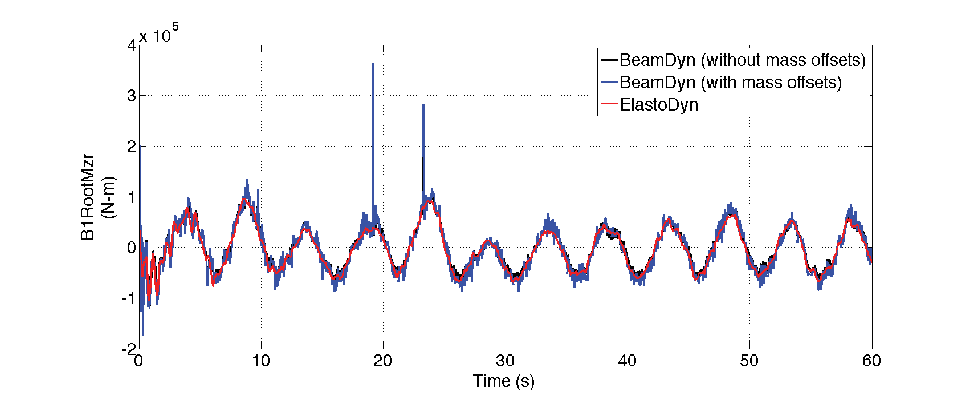
\includegraphics[width=2.8in]{EPSF/B1RootMzr.eps}
         \end{center}
    \end{itemize}
\end{frame}
%------------------------------------------------------------------------------

%------------------------------------------------------------------------------
\begin{frame}{Summary}
    \begin{itemize}
        \item Conclusion
        \begin{itemize}
        {\footnotesize
        \item Based on \alert{geometrically exact beam theory}, BeamDyn is capable of dealing with \alert{geometric nonlinear} beam problems with arbitrary magnitude of displacements and rotations for both static and dynamic analyses
        \item Along with a preprocessor like PreComp or VABS, BeamDyn takes \alert{full elastic coupling effects} into account
        \item Spectral Finite Elements and new Trapezoidal-Rule quadrature have been adopted in the implementation of BeamDyn. These new techniques further improved the efficiency and accuracy.

  \item BeamDyn is implemented following the programming requirements (data structures and interfaces) of the \alert{FAST modularization framework}. The module coupling algorithm has been implemented and verified through numerical examples.
  }
        \end{itemize}
        \item Future Work
        \begin{itemize}
            \item Introducing numerical damping to the coupling algorithm
            \item Implement modal-based method
        \end{itemize}
    \end{itemize}
\end{frame}
%------------------------------------------------------------------------------


\begin{frame}[t]{Questions?}

\tiny
\psline[linewidth=4pt,linecolor=white](-4.0,0.7)(20,0.7)

\vspace{-0.1in}
\footnotesize
\textbf{Acknowledgments}
\begin{itemize}

\item Funded by the U.S. Department of Energy under Contract No.\
DE-AC36-08-GO28308 with the National Renewable Energy Laboratory.

%\item Computing resources were provided through the NREL Computational
%Science Center, which is supported by US DOE EERE Contract
%\#DE-AC36-08GO28308.

\end{itemize}

\textbf{References}
\scriptsize
\bibliographystyle{elsarticle-harv}

\bibliography{references}

\end{frame}

\end{document}


